\subsection{Octree}

An octree is a tree data structure in which each internal node has exactly eight children. 
Octrees are often used to partition 3D space and are used in various applications such as computer graphics, computer vision, and robotics.

\begin{figure}[H]
	\centering
	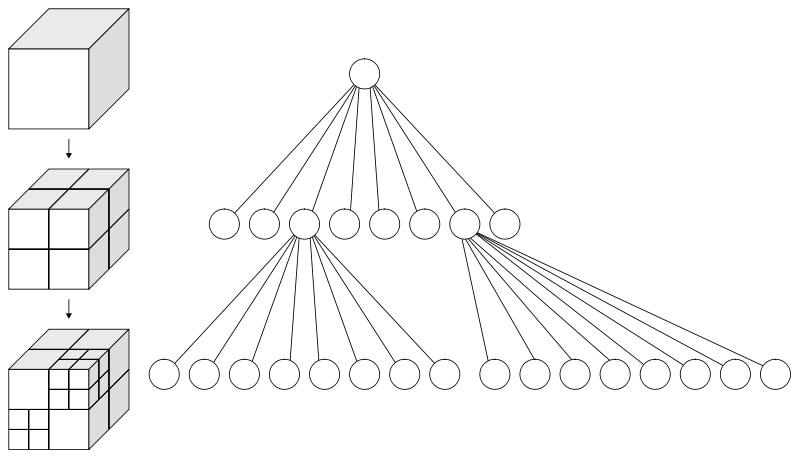
\includegraphics[width=0.5\textwidth]{octree.png}
	\caption{An example of an octree. Each cube gets recursively divided into eight equal octants. The points are stored in the leaf nodes. Image from \cite{octree_diagram}}
	\label{fig:octree}
\end{figure}

In the context of point clouds, an octree is used to partition the 3D space and store the points in the leaf nodes.
The octree is a hierarchical data structure that recursively divides 3D space into eight equal octants.
Each node in the octree represents a rectangular prism in 3D space with a particular center, width, lenghth and depth.
Nodes that aren't leaf nodes have exactly eight children, and leaf nodes store the points in the point cloud.
The root node of the octree represents the bounding box of the point cloud.
An octree has $\bigO{\log n}$ complexity for insertion and search operations, where $n$ is the number of points in the point cloud.
Bounding cubes nearest points are much finer and tighter fitting than those further away, allowing for a more accurate representation of the underlying structure of the point cloud.

Further, these tighter bounding boxes give hints on where to add new points to the point cloud, since adding points to the tighter bounding boxes will result in points that are more informative and not clustered around the original points, will not introduce any new artifacts, and will preserve the underlying structure of the point cloud.

Most octrees have a depth limit, which means that the octree will not divide the space beyond a certain depth, this is to avoid a problem of infinite recursion.
However, in our method, we do not have a depth limit, and we allow the octree to divide the space as much as possible.
since the starting point clouds are often sparse and noisy, and the lack of a depth limit allows for a more accurate representation of the underlying structure of the point cloud.
Other stops such as checking if an existing close point is already in the node are used to avoid infinite recursion.


\begin{figure}[H]
	\centering
	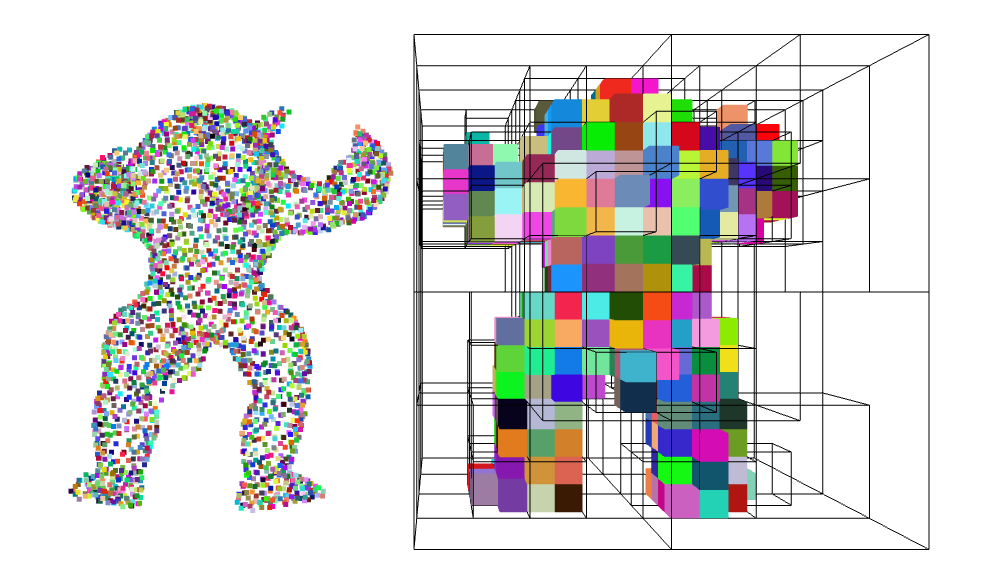
\includegraphics[width=0.5\textwidth]{octree_demo.png}
	\caption{An example of an octree with its point cloud and cubed representation. The figure was from a blog post \cite{octree_demo} and was generated using the Open3D library \cite{open3d} with a max depth of 4.}
	\label{fig:octree_depth}
\end{figure}

\subsection{Bilateral Filter}

The bilateral filter is a non-linear filter that is used to smooth images and reduce noise while preserving edges.
It is a generalization of the Gaussian filter, and it is used in various applications such as image processing, computer graphics, and computer vision.
It is defined as follows:
$$ B(I, x) = \sum\limits_{x_i \in \Omega} I(x_i) f_r(\norm{x_i - x})g_s(\norm{x_i - x})$$

In our paper, we use the bilateral filter to smooth the point cloud. Similar to the image case, the bilateral filter smooths the point cloud while preserving the edges and the underlying structure of the point cloud. It works by shifting points along a normal vector, and the amount of shift is a weighted average distance to its neighbours.
We follow Digne et al. \cite{3d_bilateral_filter_ipol} and use the following definition of the bilateral filter for point clouds:

\begin{equation} p' = p + \delta_p \cdot n_p\end{equation} 

Where $n_p$ is the normal to the regression plane of some $k$ nearest neighbours of $p$. Also following Dinge et al \cite{3d_bilateral_filter_ipol}, our implementation computes the normal with PCA. PCA will find the regression plane that fits the data best and the corresponding found eigenvectors will be orthogonal to said plane, and thus is simple to compute compared to an iterative least squares method. $\delta_p$ is the displacement of the point $p$.
The displacement is computed as follows, let $\mathcal{N}_p$ be the set of $k$ nearest neighbours of $p$:

\begin{equation}\label{eq:delta}  \delta_p = \dfrac{\sum\limits_{q \in \mathcal{N}_p} w_d(\norm{q - p})w_n(\inner{n_p}{q-p})\inner{n_p}{q-p}}{\sum\limits_{q \in \mathcal{N}_p}w_d(\norm{q - p})w_n(\inner{n_p}{q-p})}\end{equation} 

In our implementation, $w_d$ and $w_n$ are the Gaussian functions defined as follows:

\begin{equation} w_i(x) = \exp\left\{-\dfrac{x^2}{2\sigma_i^2}\right\} \label{eq:weight}\end{equation} 

In our implementation we set $\sigma_d = 0.1$ and $\sigma_n = 0.1$.
